\section{Hardware}
Der zweite wichtige Aspekt beim Aufbau eines unkonventionellen 
Supercomputers ist der physikalische Aufbau des Computers.
Hierbei muss man darauf achten ein Gleichgewicht zwischen den Faktoren 
Energieverbrauch, Rechengeschwindigkeit, und Kühlung zu finden.
Zusätzlich soll unabhängig von der Größe des Clusters eine
einfache Lösung für das Monitoring bereitgestellt werden.

\subsection{Hardwareauswahl und Motivation}
HIER NOCH INHALT EINFÜGEN! (wenn nicht redundant mit der Einleitung)


\subsection{Aufbau des Clusters}
Für ein Jetson-TK1-Cluster mit insulärer Stromversorgung
ist das Design des Racks der entscheidene Punkt um 
auch unter dauerhafter Höchstbelastung eine
stabile Funktion der Rechenknoten, zu gewährleisten.
Durch die Verwendung eines Lithium-Ion-Akkus zur Energiespeicherung
und das Risiko eines Kurzschlusses durch Kondensionswasser muss
ein geschickt aufgebautes Rechencluster gewährleisten, dass die Temperatur
der gesamten Anlage in dem Bereich von 
$18^\circ\text{C}~\text{bis}~40^\circ \text{C}$ gehalten wird. 
%Besonders beim Aufbau eines insulären Jetson-TK1-Clusters ist die Kühlung ein
%heikles Thema, da sowohl die Temperatur des Rechenclusters als auch 
%die Temperatur des Energiespeichers in seinem stark restringierten Bereich liegen müssen.
\subsubsection{Anordnung der Rechenknoten}
Hinsichtlich der oben beschriebenen Problematik ist die Anordnung der Knoten 
das zentrale Instrument mit dem man die Bildung potenzieller Wärmenester 
gegen den Platzverbrauch des Clusters abwägen kann.~\\
Wegen zu hoher Energiekosten muss auf den Einsatz einer
Wasserkühlung verzichtet werden, um eine möglichst 
hohe Energieeffizienz zu erreichen.
Die einfachsten Ansätze zum Aufbau des Supercomputers, 
welche sich mittels Luftkühlung umsetzen lassen, sind:
\begin{itemize}
\item[1)]Rechenknoten in horizontalen Schichten anzuordnen
\item[2)]Rechenknoten vertikal anzuordnen und nebeneinander aufstellen
\end{itemize} 
Je nach Aufbau ergeben sich dabei einige Vor- und Nachteile für den Großrechner, welche hier anhand der
Wärmebildern gezeigt werden.\\
~\\
\begin{minipage}{0.50\textwidth}
\centering
	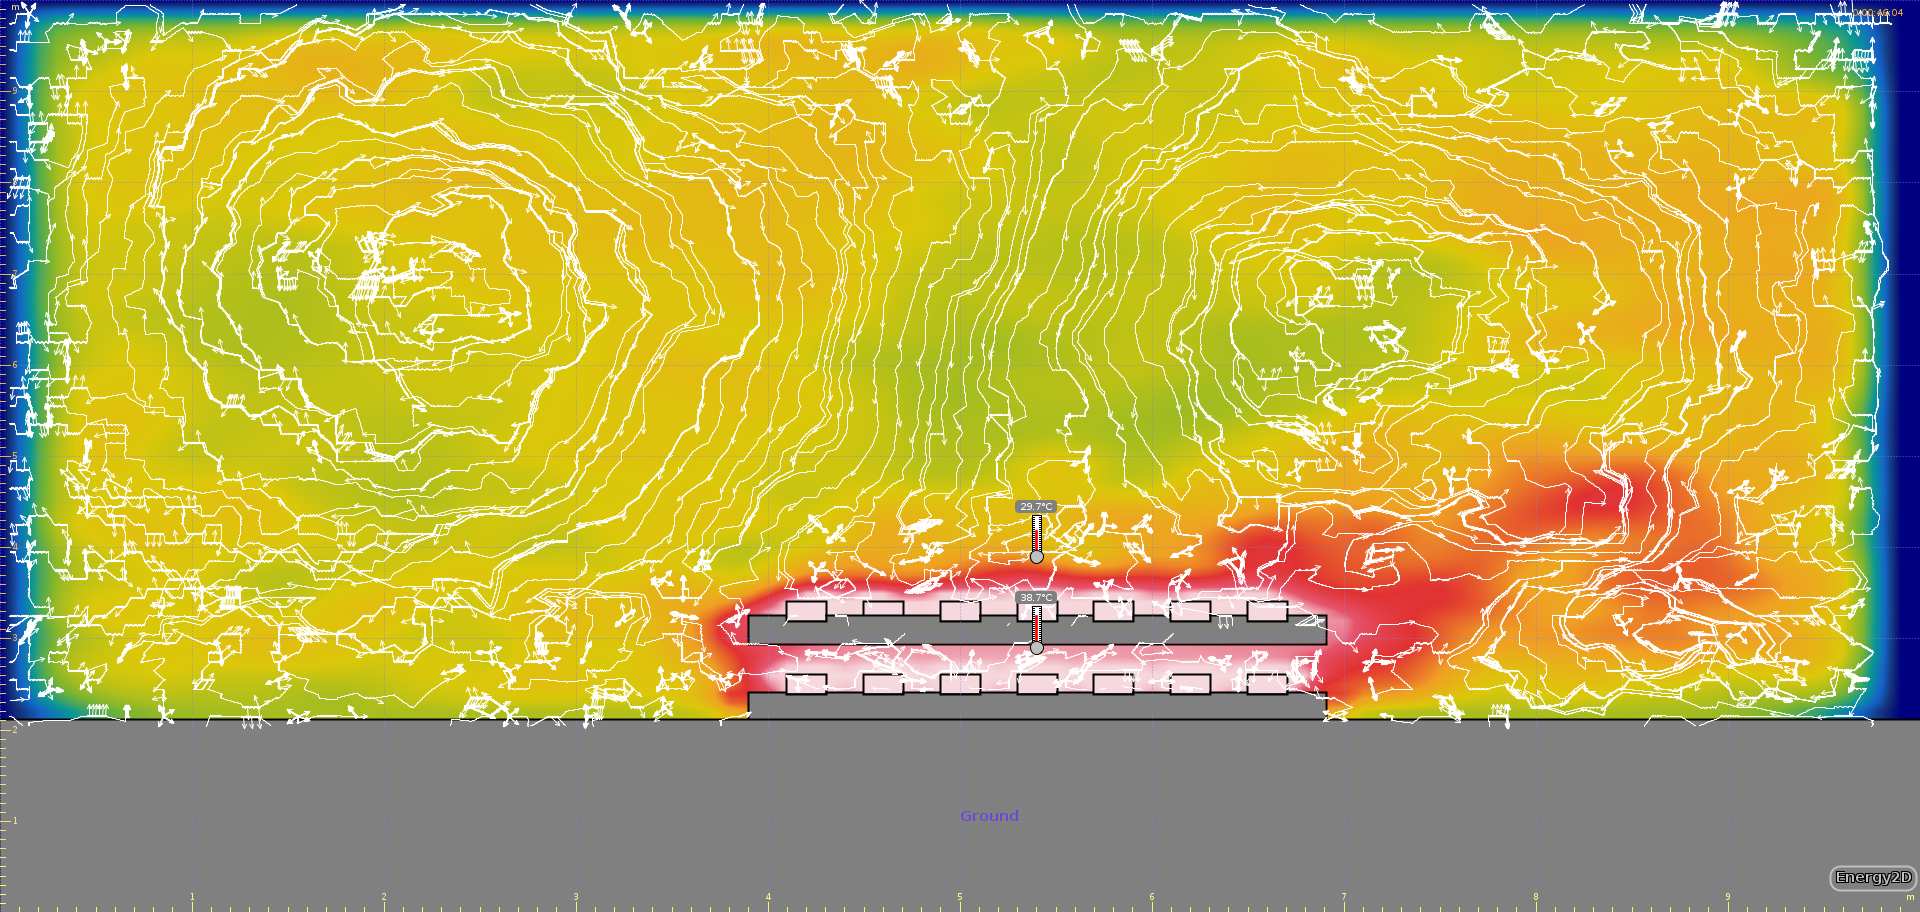
\includegraphics[width=0.99\textwidth]{./Bilder/Server-Aufbau/convective-horizontal-2.png}
	\captionof{figure}{Horizontaler Aufbau}
	\label{fig:HWPabb1}

\end{minipage}
\hfill
\begin{minipage}{0.50\textwidth}
\centering
	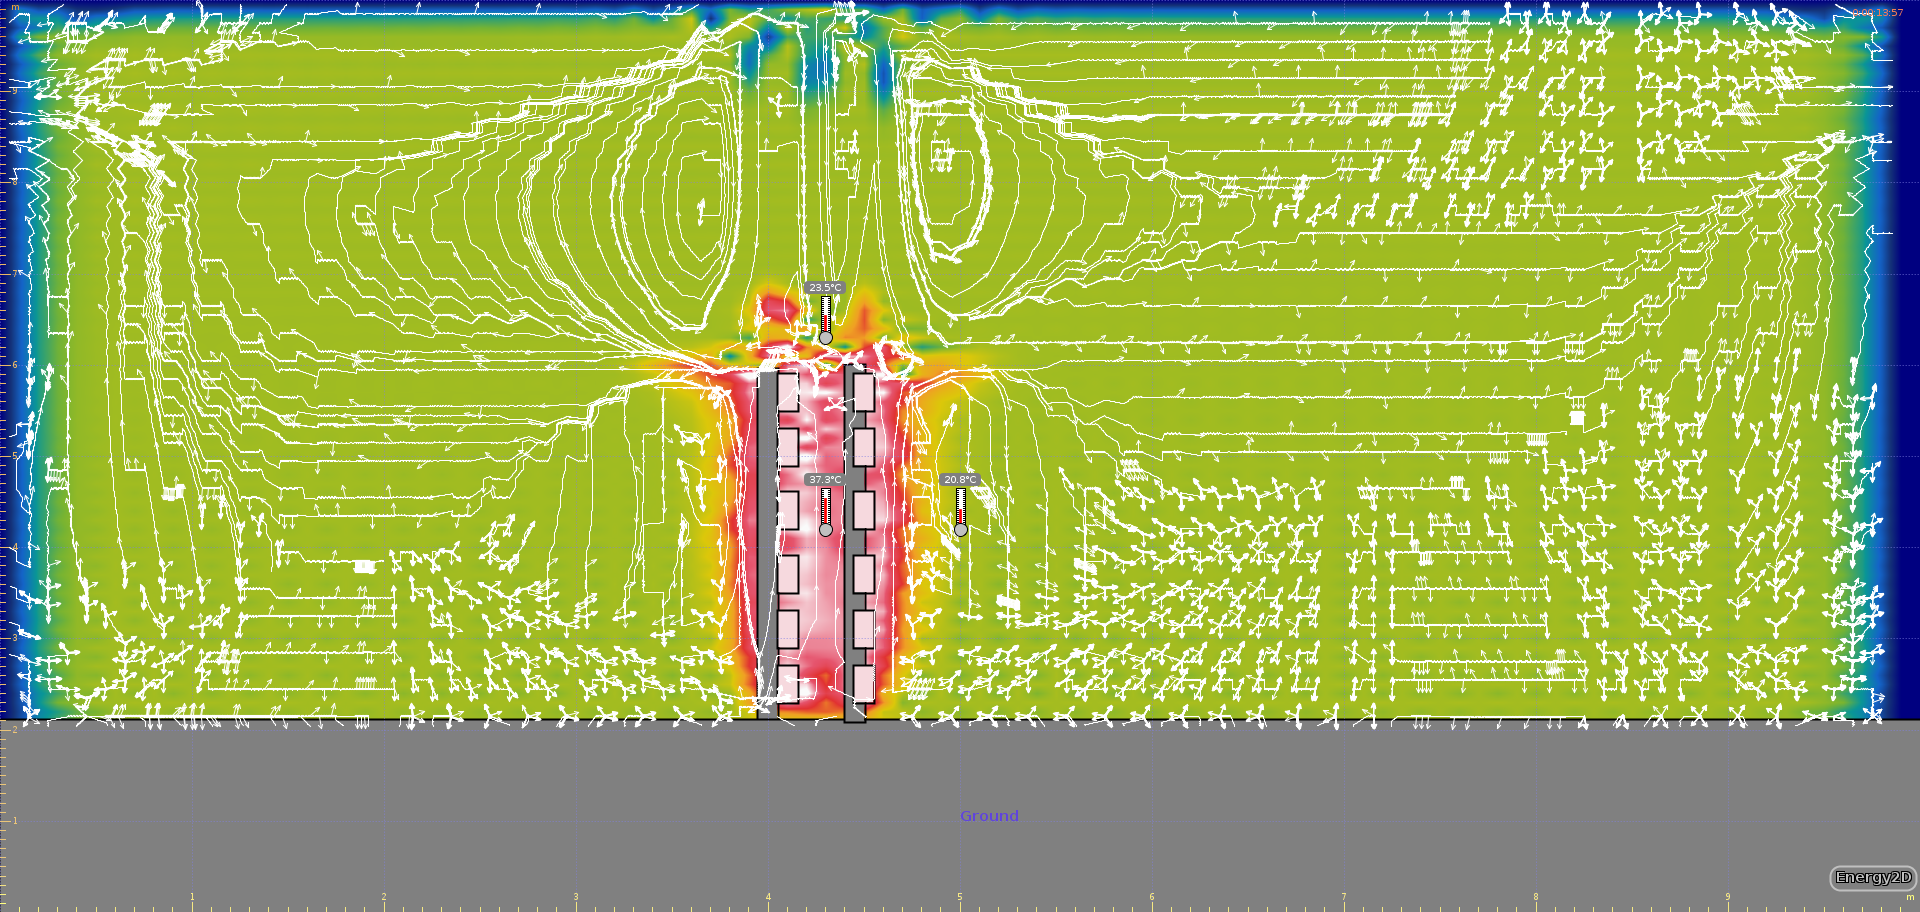
\includegraphics[width=0.99\textwidth]{./Bilder/Server-Aufbau/convective-vertical-2.png}
	\captionof{figure}{Vertikaler Aufbau}
	\label{fig:HWPabb2}
\end{minipage}
~\\
Vergleicht man diese beiden Ansätze, so sieht man, dass im horizontalen Szenario (\ref{fig:HWPabb1}) zwischen den 
Platten, auf denen die Rechenknoten angebracht sind, Wärmenester entstehen. Zudem liefert die
Analyse des Stromlinien-Diagramms, dass besonders in der Mitte der Platten die Wärme nur schlecht  
abtransportiert werden kann.\\
Im Gegensatz dazu ist der Wärmeabtransport beim vertikalem Ansatz (\ref{fig:HWPabb2}) durch aufsteigende warme Luft
besser möglich. Hierbei sollte allerdings bemerkt werden, dass durch die schiefe Lage des Ventilators
die Gravitationskraft Unregelmäßigkeiten bei der Rotation verursachen würde, was schlussendlich zu einer verkürzten Lebensdauer des Ventilators führen könnte.\\
Um die Vorteile der beiden Ansätze zu kombinieren und gleichzeitig für Wartbarkeit des 
Rechenclusters zu sorgen, wählt man einen Ansatz, bei dem die Boards in einer Doppelhelix-Struktur 
angeordnet werden.\\
~\\
\begin{minipage}{0.50\textwidth}
\centering
	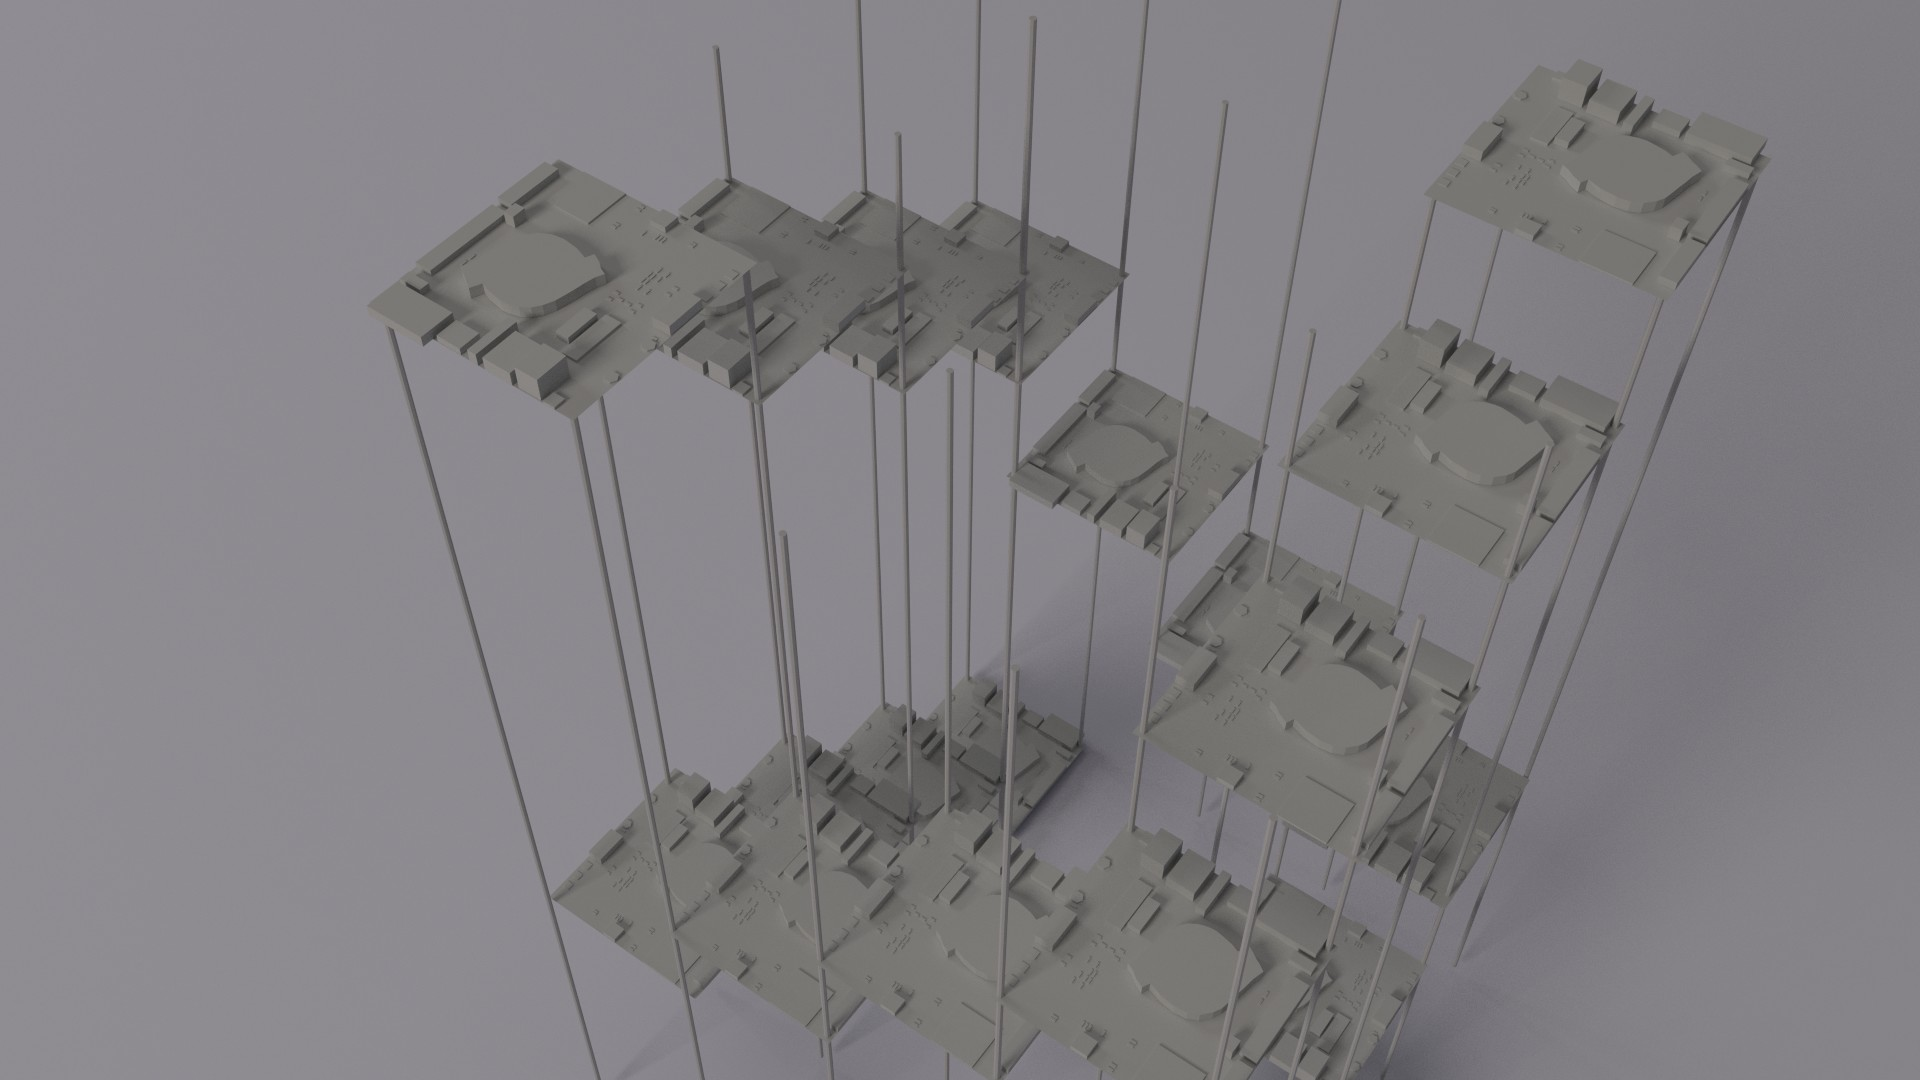
\includegraphics[width=0.99\textwidth]{./Bilder/Server-Aufbau/render3.jpg}
	\captionof{figure}{Render des Serveraufbaus}
	\label{fig:HWPabb3}
\end{minipage}
\hfill
\begin{minipage}{0.50\textwidth}
\centering
	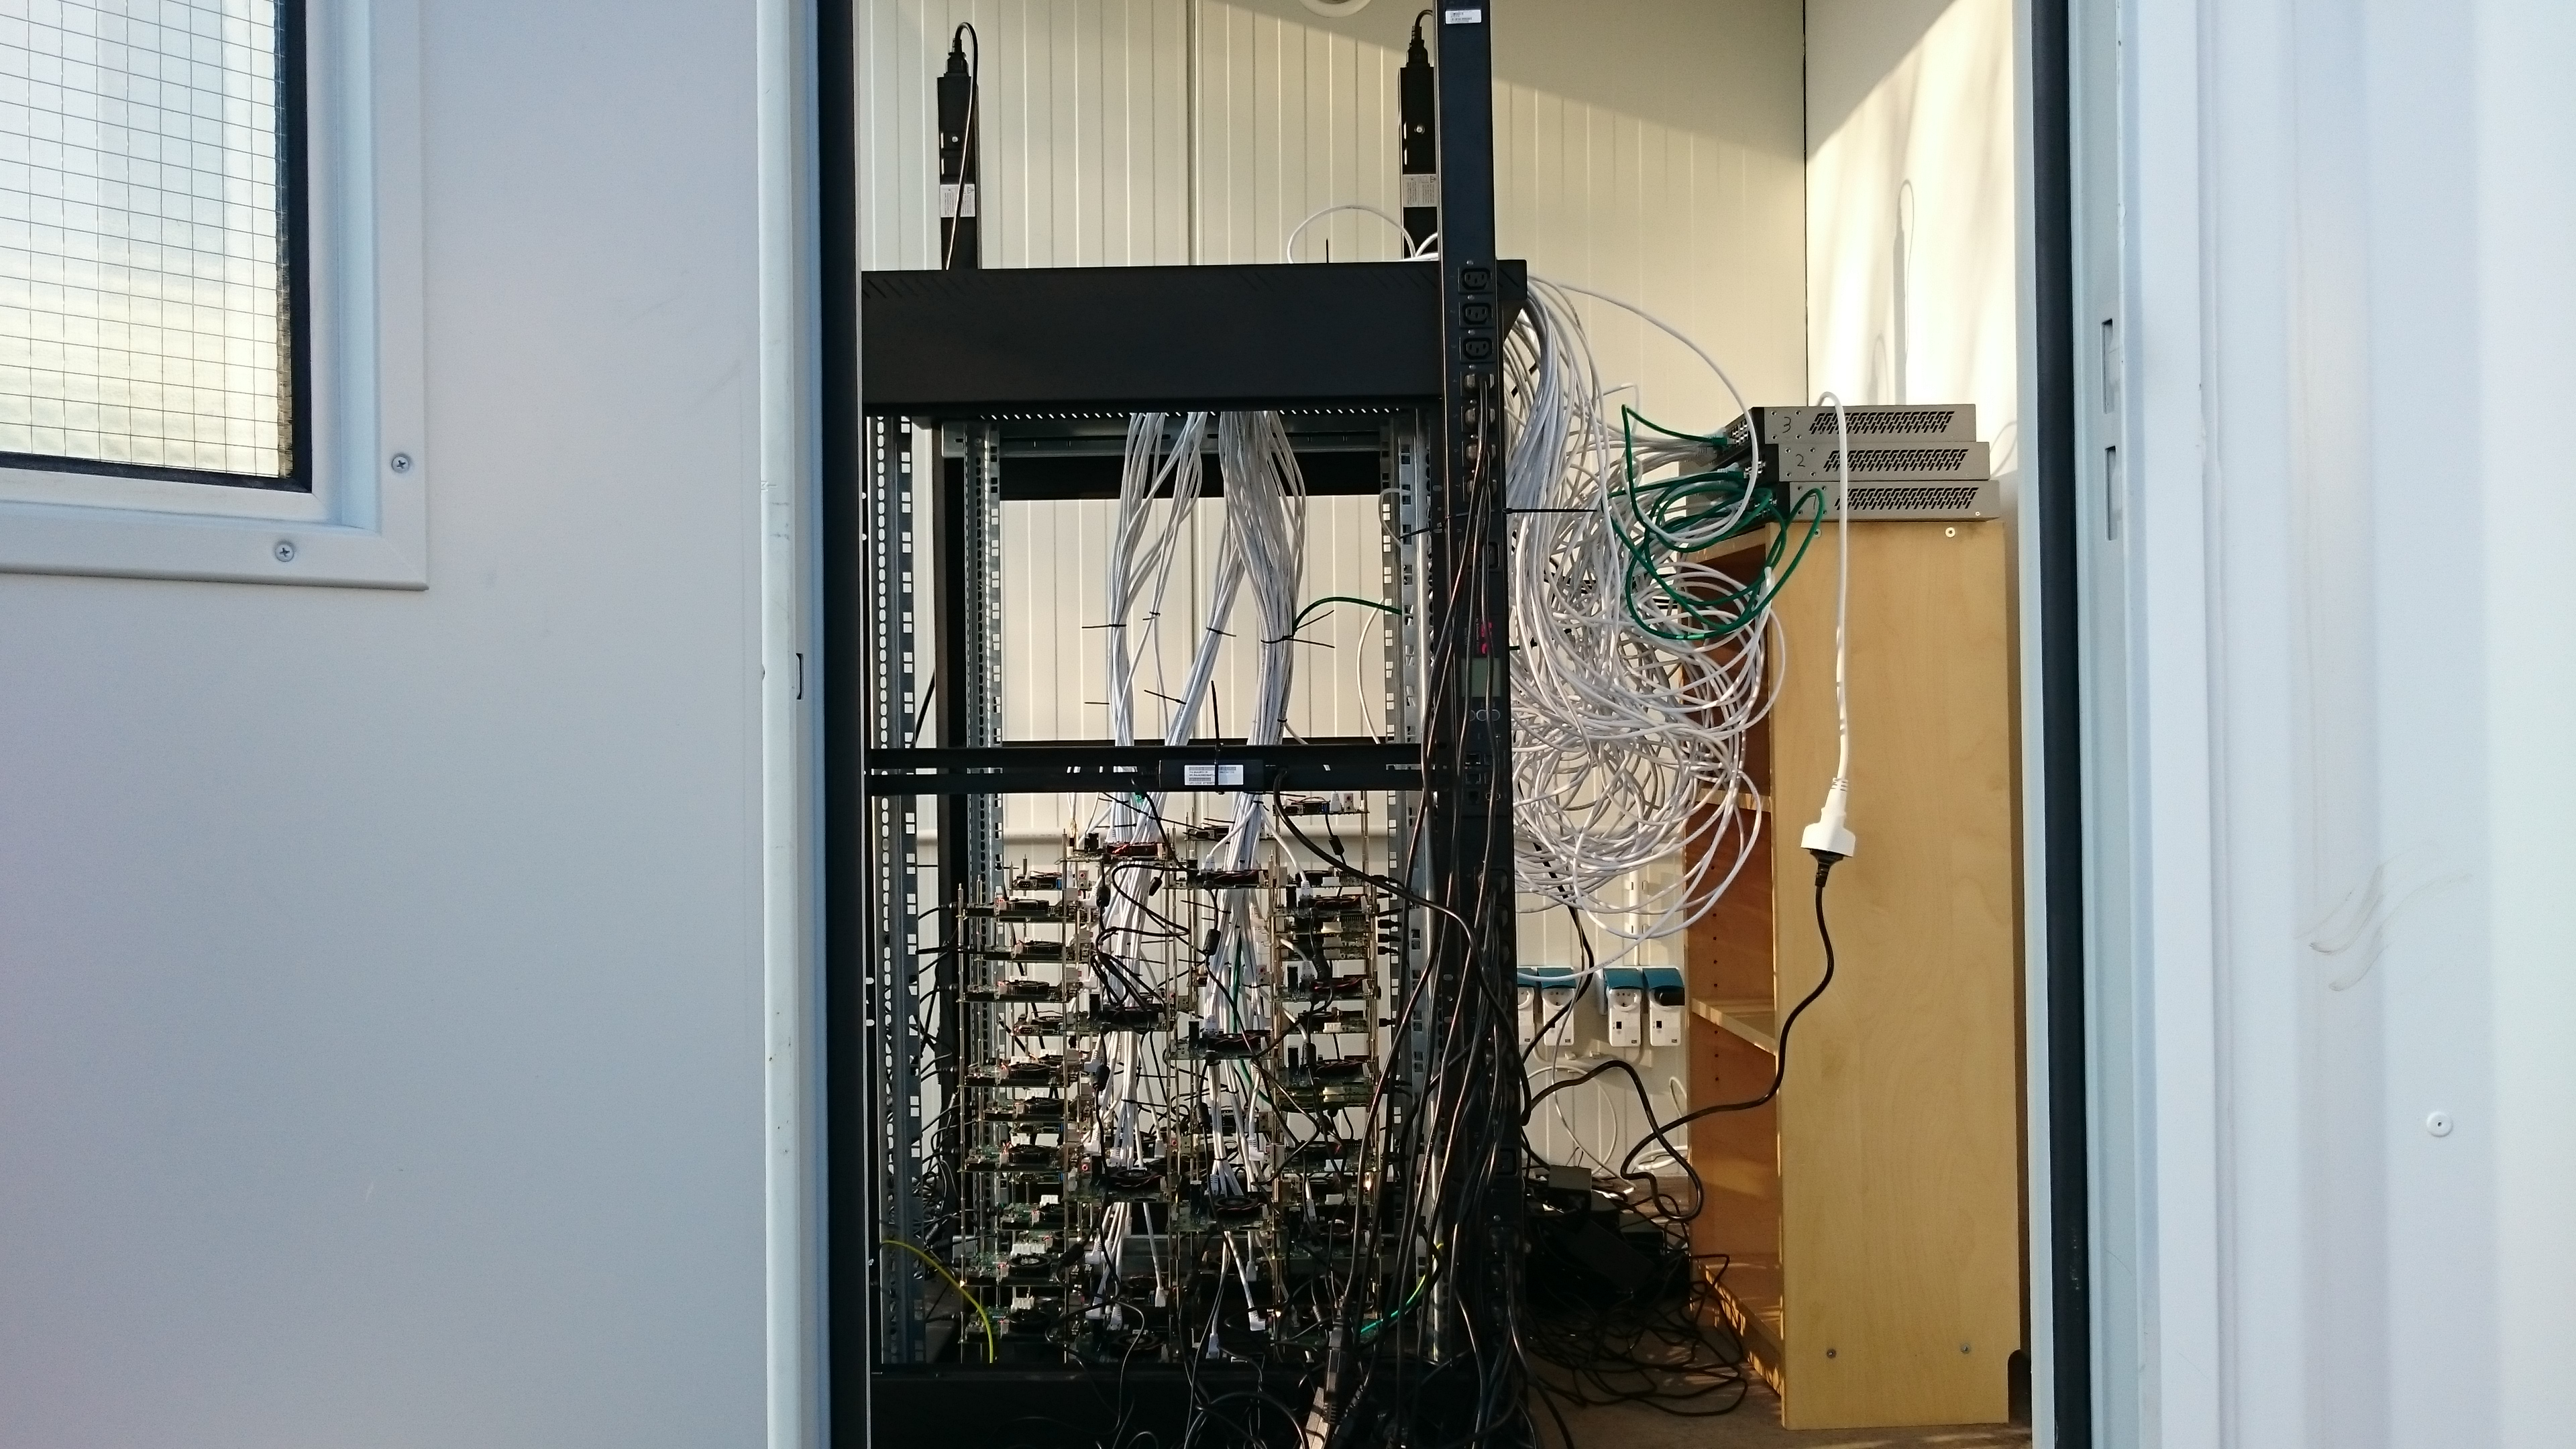
\includegraphics[width=0.99\textwidth]{./Bilder/Server-Aufbau/DSC_0020.JPG}
	\captionof{figure}{Serveraufbau (17. März 2016)}
	\label{fig:HWPabb4}
\end{minipage}
~\\
Wie auf diesen Abbildungen (\ref{fig:HWPabb3} , \ref{fig:HWPabb4}) zu erkennen ist, wird durch die Verwendung der Doppelhelix-Struktur
ein größerer Abstand zwischen den Bords für eine verbesserte Kühlung, bei gleichzeitig geringem
Platzverbrauch ermöglicht.\\ 
\subsubsection{Strom und Netzwerkanbindung}
Über die Anordnung hinaus muss nun die Stromversorgung und die Netzwerkanbindung
der Bords geregelt werden. Eine besondere Herausforderung hierbei ist die 
Anordnung der Netzteile, der einzelnen Rechenknoten. 
Um zu gewährleisten, dass sich durch das Aufheizen der Netzteile keine gefährlichen
Wärmenester bilden, wird eine spezielle Halterung verwendet.
Unter Nutzung moderner 3D-Druck Technologien, wie sie häufig in der 'Maker-Szene' eingesetzt werden,
wurde eine Halterung (\ref{fig:HWPabb5})entworfen und produziert, welche trotz geringem Materialaufwand eine sehr hohe Stabiliät 
und eine gute Luftzufuhr ermöglicht.~\\
\begin{minipage}{\textwidth}
\begin{center}
	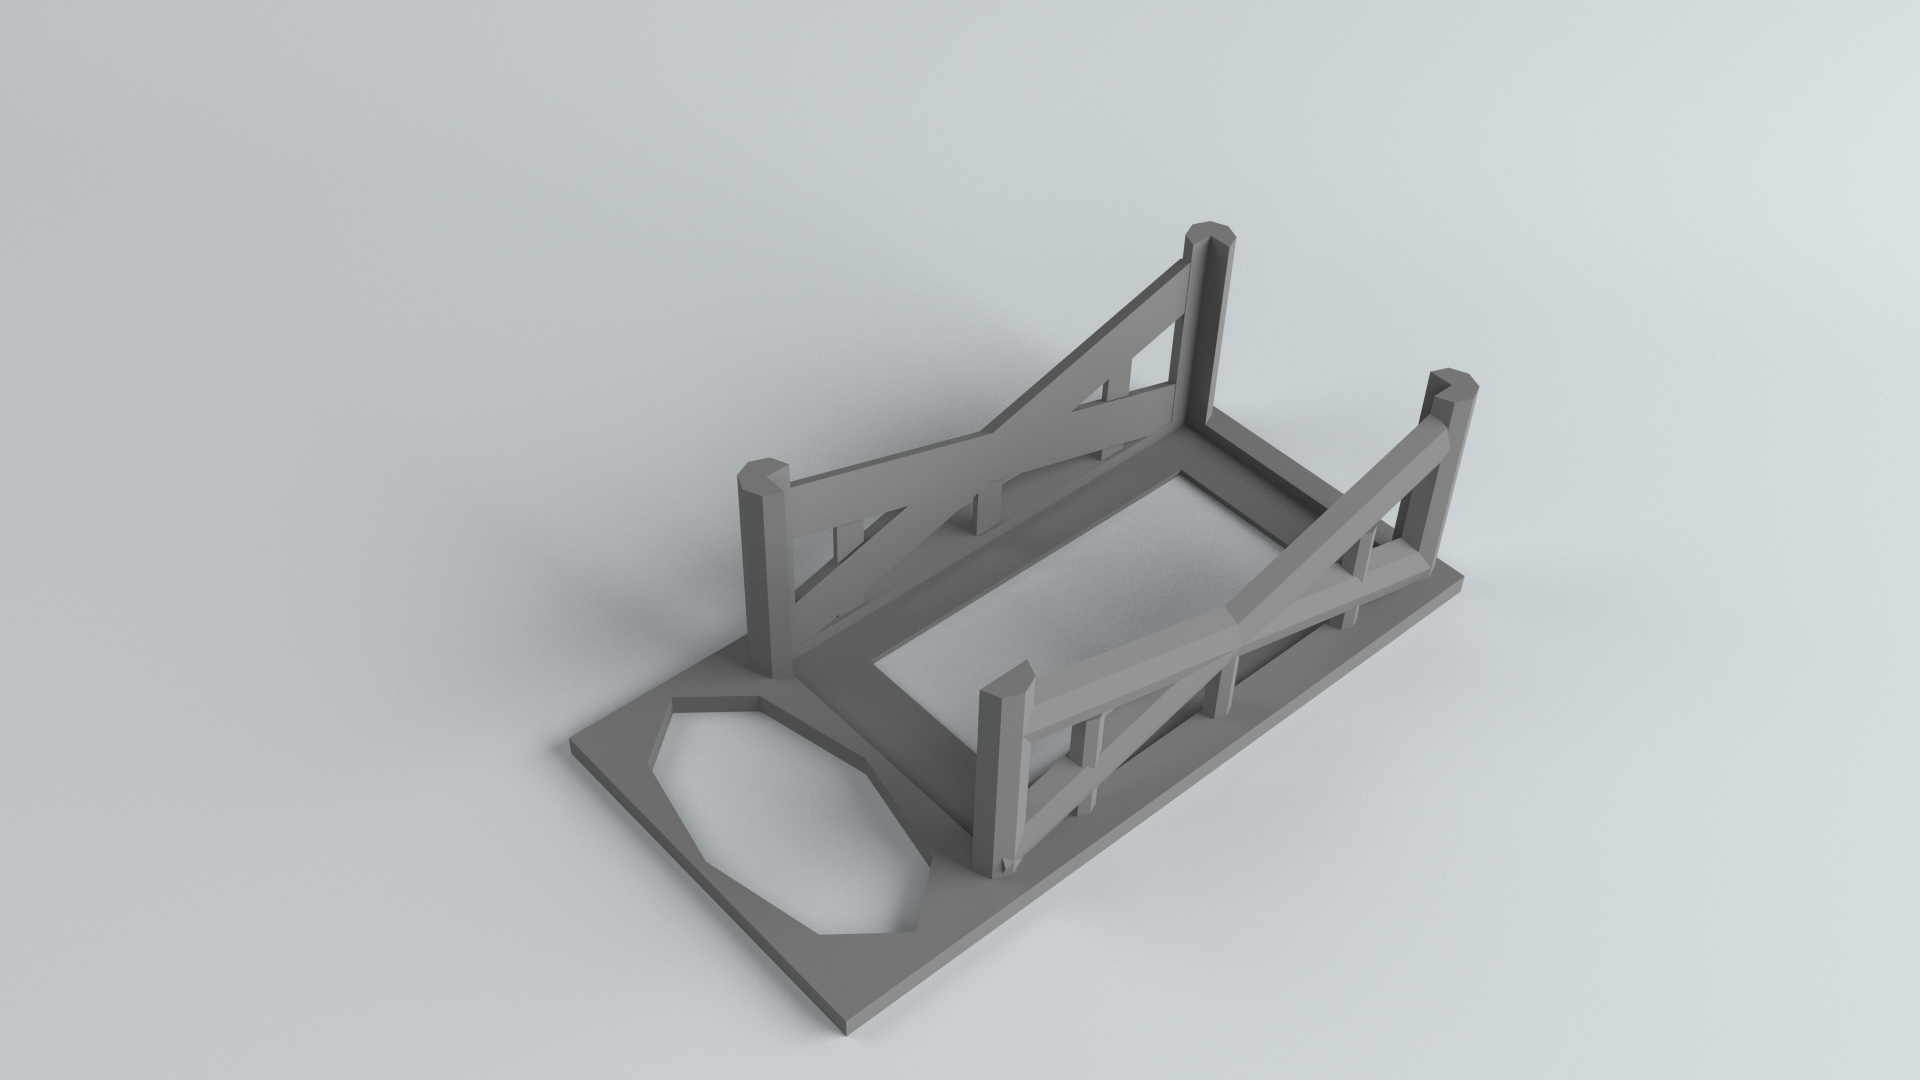
\includegraphics[width=0.7\textwidth]{./Bilder/Server-Aufbau/RenderPowerSupplyBox30.png}
	\captionof{figure}{Halterung für die Netzteile}
	%\captionof{figure}{Halterung für die Netzteile}
	\label{fig:HWPabb5}

\end{center}	
\end{minipage}
~\\

Hinsichtlich des Aspektes 'Green-Computing' ist es wichtig, ein Druckfilament zu verwenden, 
welches biokompatibel ist. Hierfür bietet sich der aus Maisstärke gewonnene Biokunststoff Polylactide (PLA) an.
Dieser hat einen Schmelzpunkt von $150^\circ\text{C}~\text{bis}~160^\circ \text{C}$
und ist daher ohne weiteres für die Halterung von Netzteilen verwendbar.


%\subsection{Wartung und Instandhaltung}
%\subsection{Dashboard} %(Ist gem dict.cc auch OK)
\subsection{Übersichtsseite}
Um das Monitoring und die Fernwartung des Clusters möglichst komfortabel zu bewerkstelligen, wurde ein Dashboard eingerichtet(\ref{fig:dashboardpic}). Hierfür ist die Hardware eines Raspberry Pi, der ersten Generation, ausreichend.
\subsubsection{Einrichtung Webserver}
Um die gemessenen Daten verwalten und darstellen zu können, wird auf dem Raspberry Pi ein LAMP-Server eingerichtet (Linux-Apache-MySQL-PHP). Die Daten werden folglich in der MySQL Datenbank abgespeichert und über PHP-Skripte ausgelesen und verarbeitet. Die Darstellung der Daten erfolgt mittels HTML, CSS und Javascript. Des Weiteren muss der Raspberry Pi so konfiguriert werden, dass erstens das Webinterface von außen einsehbar ist, und vor allem, dass auch von außen in die Datenbank geschrieben werden kann.

\begin{minipage}{\textwidth}

\begin{center}
	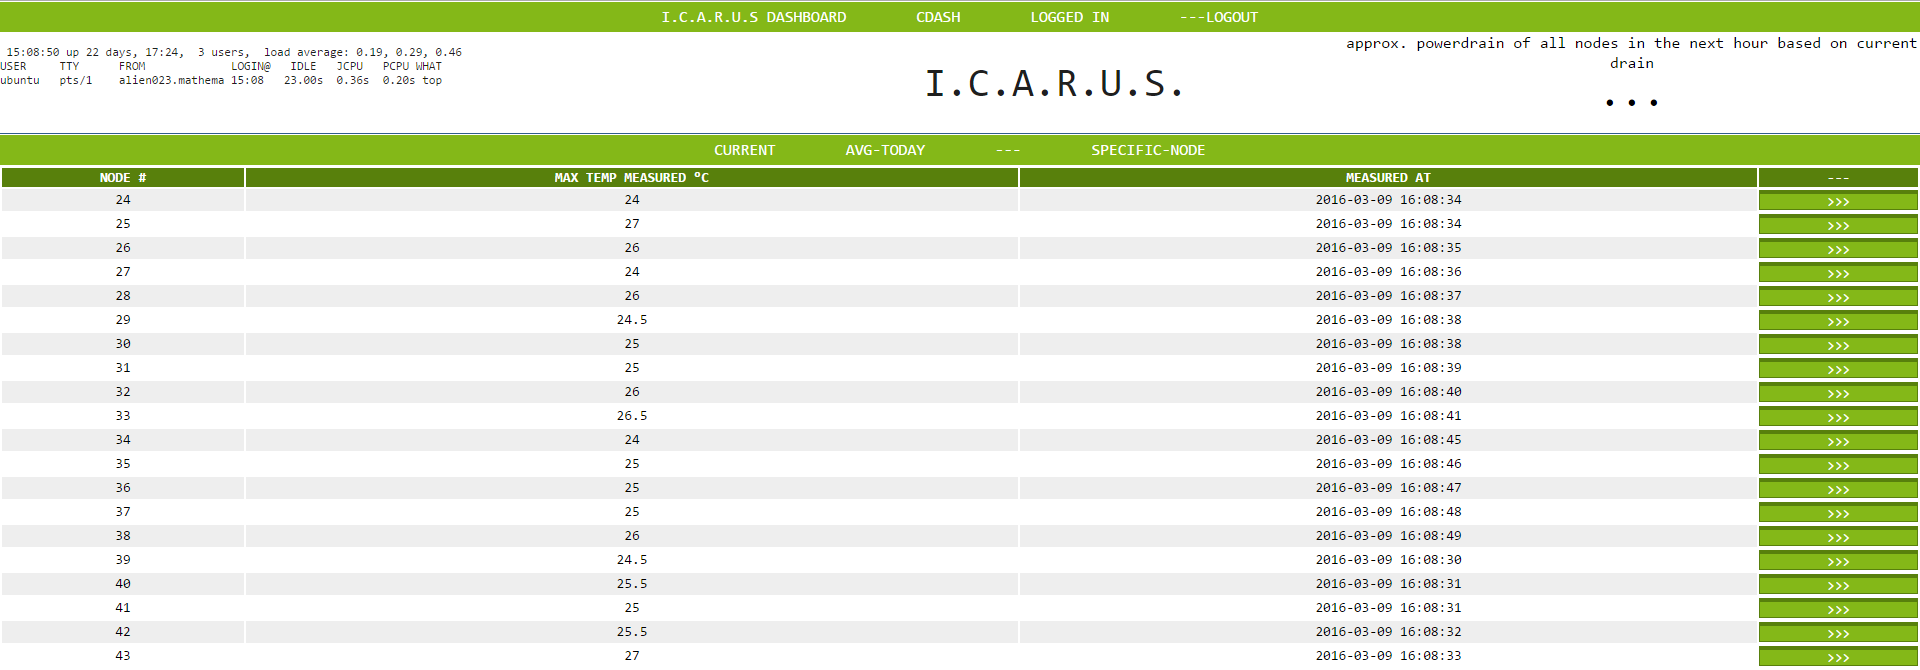
\includegraphics[width=0.7\textwidth]{./Bilder/Dashboard/Dashboard_frontend.png}
		\captionof{figure}{Dashboard Frontend}
	\label{fig:dashboardpic}

\end{center}	
\end{minipage}

\subsubsection{Sammeln der Messdaten}
Die Temperaturen können lokal auf den einzelnen Boards ausgelesen werden. Dies wird verwendet, um mittels C++ ein Programm laufen zu lassen, welches sich auf den einzelnen Rechenknoten nacheinander einloggt, die Temperatur Daten an verschiedenen Stellen des Jetson-Boards ausliest und anschließend zusammen in die MySQL-Datenbank auf dem Webserver einfügt.\\
Um die restringierte Hardware des Raspberry Pi's nicht zu überlasten, wird das Programm auf dem Gateway-Knoten des Clusters ausgeführt, weshalb der oben genannte Zugriff von außen des Raspberry Pi's wichtig ist. \\
Um qualitative Aussagen über die Energieeffizienz machen zu können wurde eine PDU angeschafft, mit welcher der Stromverbrauch der einzelnen Knoten messbar gemacht werden sollte. \\
--- kleiner Text bzgl alternativer Messmethoden folgt nach Donnerstag nach Gespräch mit Markus---\\

\subsubsection{Weitere Funktionen des Dashboards}
Die Aufgabe der Übersichtsseite beschränkt sich nicht nur auf das Sammeln und Anzeigen der Daten. Es soll auch die Fernwartung der einzelnen Knoten bezüglich der Stromzufuhr geregelt werden. Dies soll mittels SSH-Zugriff auf die PDUs bewerkstelligt werden, ist jedoch zur Veröffentlichung dieses Berichts noch in Entwicklung.
Des Weiteren wird ebenfalls mittels SSH-Zugriff und elementaren Linux-Befehlen die aktuell am Cluster angemeldeten Nutzer, sowie deren aktuell ausgeführten Programme, angezeigt.
